\documentclass[12pt, oneside]{report}\usepackage[]{graphicx}\usepackage[]{color}
% maxwidth is the original width if it is less than linewidth
% otherwise use linewidth (to make sure the graphics do not exceed the margin)
\makeatletter
\def\maxwidth{ %
  \ifdim\Gin@nat@width>\linewidth
    \linewidth
  \else
    \Gin@nat@width
  \fi
}
\makeatother

\usepackage{Sweavel}


\usepackage[margin=0.85in]{geometry}
\linespread{1}
\usepackage{xcolor}
\usepackage[colorlinks=false, linkbordercolor=white, citebordercolor=white, 
    filebordercolor=white, urlbordercolor=white]{hyperref}
    
\usepackage{graphicx}
\usepackage[utf8]{inputenc}
\usepackage[english]{babel}
\usepackage[T1]{fontenc}

\usepackage{fancyhdr}
\pagestyle{fancy}
\renewcommand{\headrulewidth}{0.4pt}
\fancyhead{}
  \fancyhead[L]{Statistics for Computer Science -- assignment 1} %%% change to your course name and change the number accordingly
\fancyhead[R]{Kanitha Chim} %%% change to your first name and surname
\fancyfoot{}
\fancyfoot[C]{\thepage}

\usepackage{titlesec}
\titlespacing{\chapter}{0pt}{*4}{*2.5}

\titleformat{\chapter}{\normalfont\huge\bf}{\thechapter}{20pt}{\huge\bf}


% Setting up of environment
\usepackage{listings}
\definecolor{dgray}{gray}{0.35} % colour of comments
\definecolor{lgray}{gray}{0.95} % background colour of R-code
\definecolor{llgray}{gray}{0.98} % background colour of R-outputs

\lstdefinestyle{Rstyle}{ % settings of R-code style
language=R, % setting language R
basicstyle=\ttfamily\small, % font and size of R-code
backgroundcolor=\color{lgray}, % background colour of R-code
commentstyle=\ttfamily\small\itshape\color{dgray}, % colour of R comments
showstringspaces=false, % forbidding the highlighting of spaces
numbers=left, % numbering on the left
numberstyle=\ttfamily\small, % font and size of numbering
stepnumber=1, % numbering with step 1
firstnumber=last, % cumulative numbering of rows in consecutive Chunks
breaklines=T} % automatic line breaks of code at the end of a line

\lstdefinestyle{Routstyle}{ %  settings of R-output style
language=R, % setting language R
basicstyle=\ttfamily\small, % font and size of R-output
backgroundcolor=\color{llgray}, % background colour of R-code
showstringspaces=false, % forbidding the highlighting of spaces
numbers=right, % numbering on the right
numberstyle=\ttfamily\small, % font and size of numbering
firstnumber=last, % cumulative numbering of rows in consecutive Chunks
breaklines=T} % automatic line breaks of code at the end of a line

\begin{document}



\begin{titlepage}
    \begin{center}
        \vspace*{1cm}
        
        \Huge
          \textbf{Statistics for Computer Science} %%% change to your course name
        
        \vspace{0.5cm}
        \LARGE
        Assignment 1 %%% change the number accordingly
        
        \vspace{1.5cm}
        
        \textbf{Kanitha Chim} %%% change to your first name and surname
   		  \vspace{1.5cm}
        
        \textbf{501453} %%% change to your UCO
       
        \vfill
        
        Field of Study Software System and Service Management %%% change to your field of study
        
        \vspace{0.8cm}
          \Large
        Faculty of Informatics\\
        Masaryk University\\
        \vspace{0.5cm}
       \today
        
    \end{center}
\end{titlepage}

\addtocontents{toc}{~\hfill\textbf{Page}\par}

\section*{Exercise 1}
\noindent 1. Create your own R-functions for calculating estimates of the following characteristics: sample
mean, sample five number summary, sample skewness, sample kurtosis, sample variance, sample
standard deviation, sample range, sample decile range, sample 0.1-trimmed average and sample
0.1-trimmed variance. Use Cramér’s estimates for skewness and kurtosis. Do not use in-
built functions min(), max(), mean(), quantile(), var(), sd(), range() or functions from external
libraries.

\subsection*{Implementation in R}

\begin{Schunk}
\begin{Sinput}
#function to calculate minimum
cal_minimum <- function(x){
  x <- sort(x)
  min_val <- x[1]
  return(min_val)
}

#function to calculate maximum
cal_maximum <- function(x){
  x <- sort(x)
  max_val <- tail(x,1)
  return(max_val)
}

#median, first quartile, thrid quartile, quartile_type should be, one, two(median), or three
cal_quartile <- function(x, quartile_type){
  x <- sort(x)
  result <- 0
  
  if(quartile_type == 'two'){
    if(length(x) %% 2 == 0){
      return((x[length(x)/2] + x[length(x+1)/2])/2)
    }else{
      return(x[length(x+1)/2])
    }
  }else if(quartile_type == 'one'){
    position <- (length(x) + 1)/4
    if (floor(position) == ceiling(position)){
      return(x[position])
    }else{
      return((x[floor(position)] + x[ceiling(position)])/2)
    }
  }else if(quartile_type == 'three'){
    position <- (3*(length(x) + 1))/4
    if (floor(position) == ceiling(position)){
      return(x[position])
    }else{
      return((x[floor(position)] + x[ceiling(position)])/2)
    }
  }
}

#Sample mean
cal_mean <- function(x){
  result <- sum(x) / length(x)
  return(result)
}

#Sample five number summary
cal_five_num_summary <- function(x){
  min <- cal_minimum(x)
  q1 <- cal_quartile(x, 'one')
  q2 <- cal_quartile(x, 'two')
  q3 <- cal_quartile(x, 'three')
  max <- cal_maximum(x)
  return(c(min, q1, q2, q3, max))
}

#Sample Skewness
cal_coef_skew <- function(x){
  s <- sqrt(cal_sample_variance(x))
  mean <- cal_mean(x)
  total <- 0
  for(i in x){
    total = total + (i - mean)^3
  }
  return(total/(s^3 * length(x)))
}

#Sample Kurtosis
cal_coef_kurt <- function(x){
  s <- sqrt(cal_sample_variance(x))
  mean <- cal_mean(x)
  total <- 0
  for(i in x){
    total = total + (i - mean)^4
  }
  total = total/(s^4 * length(x))
  return(total -3)
}

#Sample Variance
cal_sample_variance <- function(x){
  mean <- cal_mean(x)
  n_minus_one <- length(x) - 1
  total <- 0
  for(i in x){
    total = total + (i - mean)^2
  }
  return(total/n_minus_one)
}

#Sample Standard Deviation
cal_sd <- function(x){
  sample_variance <- cal_sample_variance(x)
  return(sqrt(sample_variance))
}

#Sample Range
cal_sample_range <- function(x){
  return(cal_maximum(x) - cal_minimum(x))
}

#Sample Decile Range
cal_sample_decile_range <- function(x){
  x_0.9 <- 90/100 * (length(x) +1)
  x_0.1 <- 10/100 * (length(x) +1)
  
  if (floor(x_0.9) == ceiling(x_0.9)){
    x_0.9 = x_0.9
  }else{
    x_0.9 = (x[floor(x_0.9)] + x[ceiling(x_0.9)])/2
  }
  
  if (floor(x_0.1) == ceiling(x_0.1)){
    x_0.1 = x_0.1
  }else{
    x_0.1 = (x[floor(x_0.1)] + x[ceiling(x_0.1)])/2
  }
  return(x_0.9 - x_0.1)
}

#Sample 0.1 trimmed average
cal_sample_0.1_trimmed_average <- function(x){
  g <- abs(0.1 * length(x))
  n <- length(x)
  total <- 0
  for(i in seq(g+1, n-g, 1)){
    total <- total + x[i]
  }
  return(total/(n - 2*g))
}

#Sample 0.1 trimmed variance
cal_sample_0.1_trimmed_variance <- function(x){
   g <- abs(0.1 * length(x))
   n <- length(x)
   x_gt <- cal_sample_0.1_trimmed_average(x)
   total <- 0
   for(i in seq(g+1, n-g, 1)){
     total <- total + (x[i] - x_gt)^2
   }
   return(total/(n - 2*g - 1))
}

library(xtable)
\end{Sinput}
\end{Schunk}

\noindent 2. Separately for each population calculate sample size and these characteristics of maximum cranial breadth. Print them in a table with values rounded to 4 decimal places.

\subsection*{Implementation in R}
\begin{Schunk}
\begin{Sinput}
setwd(getwd())
Howell <- read.csv('Howell.csv')
Howell.Male <- Howell[Howell$Sex == 'M', ]
Howell.Male.Australi <- Howell.Male[(Howell.Male$Population == 'AUSTRALI'), ]
Howell.Male.Peru <- Howell.Male[(Howell.Male$Population == 'PERU'), ]

#Working on population of 'AUSTRALI'
Australi.sample_size <- length(Howell.Male.Australi$XCB)
Australi.sample_mean <- cal_mean(Howell.Male.Australi$XCB)
Australi.sample_five_num_summary <- cal_five_num_summary(Howell.Male.Australi$XCB)
Australi.sample_skewness <- cal_coef_skew(Howell.Male.Australi$XCB)
Australi.sample_kurtosis <- cal_coef_kurt(Howell.Male.Australi$XCB)
Australi.sample_variance <- cal_sample_variance(Howell.Male.Australi$XCB)
Australi.sample_sd <- cal_sd(Howell.Male.Australi$XCB)
Australi.sample_range <- cal_sample_range(Howell.Male.Australi$XCB)
Australi.sample_decile_range <- cal_sample_decile_range(Howell.Male.Australi$XCB)
Australi.sample_0.1_trimmed_average <- cal_sample_0.1_trimmed_average(Howell.Male.Australi$XCB)
Australi.sample_0.1_trimmed_variance <- cal_sample_0.1_trimmed_variance(Howell.Male.Australi$XCB)

#Working on population of 'PERU'
Peru.sample_size <- length(Howell.Male.Peru$XCB)
Peru.sample_mean <- cal_mean(Howell.Male.Peru$XCB)
Peru.sample_five_num_summary <- cal_five_num_summary(Howell.Male.Peru$XCB)
Peru.sample_skewness <- cal_coef_skew(Howell.Male.Peru$XCB)
Peru.sample_kurtosis <- cal_coef_kurt(Howell.Male.Peru$XCB)
Peru.sample_variance <- cal_sample_variance(Howell.Male.Peru$XCB)
Peru.sample_sd <- cal_sd(Howell.Male.Peru$XCB)
Peru.sample_range <- cal_sample_range(Howell.Male.Peru$XCB)
Peru.sample_decile_range <- cal_sample_decile_range(Howell.Male.Peru$XCB)
Peru.sample_0.1_trimmed_average <- cal_sample_0.1_trimmed_average(Howell.Male.Peru$XCB)
Peru.sample_0.1_trimmed_variance <- cal_sample_0.1_trimmed_variance(Howell.Male.Peru$XCB)

Howell.characteristics <- data.frame(Australi=c(Australi.sample_size, 
                        Australi.sample_mean, 
                        Australi.sample_five_num_summary, 
                        Australi.sample_skewness, 
                        Australi.sample_kurtosis, 
                        Australi.sample_variance, 
                        Australi.sample_sd, 
                        Australi.sample_range, 
                        Australi.sample_decile_range, 
                        Australi.sample_0.1_trimmed_average, 
                        Australi.sample_0.1_trimmed_variance),
                  Peru=c(Peru.sample_size, Peru.sample_mean, 
                         Peru.sample_five_num_summary, 
                         Peru.sample_skewness, 
                         Peru.sample_kurtosis, 
                         Peru.sample_variance, 
                         Peru.sample_sd, 
                         Peru.sample_range, 
                         Peru.sample_decile_range, 
                         Peru.sample_0.1_trimmed_average, 
                         Peru.sample_0.1_trimmed_variance),
                  row.names = c('Size', 'Mean', 'Minimum', 
                                'Q1', 'Q2', 'Q3', 'Maximum', 
                                'Skewness', 'Kurtosis', 
                                'Variance', 'Standard Deviation', 
                                'Range', 'Decile Range', 
                                'Sampe 0.1 trimmed average', 
                                'Sample 0.1 trimmed variance'))

library(xtable)
\end{Sinput}
\end{Schunk}

\noindent 3. Create boxplots of maximum cranial breadth of each population side by side in one figure. Set the width of boxes to be proportional to sample sizes, add notches and arithmetic averages for both groups.

\subsection*{Implementation in R}
\begin{Schunk}
\begin{Sinput}
max.len = max(length(Howell.Male.Australi$XCB), length(Howell.Male.Peru$XCB))
x=c(Howell.Male.Australi$XCB, rep(NA, max.len - length(Howell.Male.Australi$XCB)))
y=c(Howell.Male.Peru$XCB, rep(NA, max.len - length(Howell.Male.Peru$XCB)))

Populations <- c('Australi', 'Peru')
values <- c(x, y)
df <- data.frame(Populations, values)

library(ggplot2)
boxplot <- ggplot(df, aes(x=Populations, y=values, fill=Populations)) +
          geom_boxplot(notch = TRUE, width=(55/110)) +
          scale_fill_manual(values=c("lightblue", "lightgreen")) +
          ylab('Maximum cranial breadth') +
          xlab('Populations') +
          annotate("text", x=1, y=Australi.sample_mean, 
                   label= round(Australi.sample_mean, 4)) +
          annotate("text", x=2, y=Peru.sample_mean, 
                   label= round(Peru.sample_mean, 4)) +
          ggtitle('Boxplot of maximum cranial breadth') +
          theme(plot.title = element_text(hjust = 0.5))
\end{Sinput}
\end{Schunk}

\noindent 4. Separately for each population create histogram of maximum cranial breadth. Make sure that the histograms can be easily compared (without using back-to-back histogram).
\subsection*{Implementation in R}
\begin{Schunk}
\begin{Sinput}
Australi.hist <- ggplot(data=data.frame(Australi=c(Howell.Male.Australi$XCB)), 
                        aes(x=Howell.Male.Australi$XCB)) + 
                geom_histogram(color="darkblue", fill="lightblue", binwidth = 1) + 
                xlab('Maximum cranial breadth of Australi') +
                ylab('Frequecy') +
                scale_x_continuous(breaks = seq(124, 144, 2), lim = c(122, 146)) + 
                geom_text(stat = 'count', aes(label =..count.., vjust = -0.5))

Peru.hist <- ggplot(data=data.frame(Peru=c(Howell.Male.Peru$XCB)), 
                    aes(x=Howell.Male.Peru$XCB)) + 
            geom_histogram(color="darkgreen", fill="lightgreen", binwidth = 1) + 
            xlab('Maximum cranial breadth of Peru') + 
            ylab('Frequency') +
            scale_x_continuous(breaks = seq(129, 149, 2), lim = c(128, 150)) + 
            geom_text(stat = 'count', aes(label =..count.., vjust = -0.5))
\end{Sinput}
\end{Schunk}


\noindent 5. Create normal qq-plot of maximum cranial breadth for each population.
\subsection*{Implementation in R}
\begin{Schunk}
\begin{Sinput}
Australi.qq <- ggplot(data=data.frame(Australi=c(Howell.Male.Australi$XCB))) + 
                aes(sample= Australi) + 
                geom_qq(distribution = qnorm) + 
                geom_qq_line(line.p = c(0.25, 0.75), col = "lightblue") + 
                ylab('Maximum cranial breadth for Australi') + 
                ggtitle('QQ-Plot of maximum cranial breadth of Australi') + 
                theme(plot.title = element_text(hjust = 0.5))

Peru.qq <- ggplot(data=data.frame(Peru=c(Howell.Male.Peru$XCB))) + 
            aes(sample= Peru) + 
            geom_qq(distribution = qnorm) + 
            geom_qq_line(line.p = c(0.25, 0.75), col = "lightgreen") + 
            ylab('Maximum cranial breadth for Peru') + 
            ggtitle('QQ-Plot of maximum cranial breadth of Peru') + 
            theme(plot.title = element_text(hjust = 0.5))
\end{Sinput}
\end{Schunk}

\noindent 6. Interpretion of results and graphics. \\

\begin{center}
\textbf {Characteristics of maximum cranial breadth} \\
\end{center}
Table represents the characteristics of maximum cranial breadth. The selected populations are male people from Austali and Peru.
% latex table generated in R 3.6.3 by xtable 1.8-4 package
% Mon Apr 13 17:38:16 2020
\begin{table}[ht]
\centering
\begin{tabular}{|l|l|l|}
  \hline
 & Australi & Peru \\ 
  \hline
Size &  52.0000 &  55.0000 \\ 
  Mean & 131.9423 & 137.9455 \\ 
  Minimum & 124.0000 & 129.0000 \\ 
  Q1 & 128.0000 & 135.0000 \\ 
  Q2 & 131.0000 & 138.0000 \\ 
  Q3 & 134.0000 & 141.0000 \\ 
  Maximum & 144.0000 & 149.0000 \\ 
  Skewness &   0.6436 &  -0.0037 \\ 
  Kurtosis &  -0.3390 &   0.0616 \\ 
  Variance &  26.0554 &  15.8673 \\ 
  Standard Deviation &   5.1045 &   3.9834 \\ 
  Range &  20.0000 &  20.0000 \\ 
  Decile Range &  15.0000 &  -4.0000 \\ 
  Sampe 0.1 trimmed average & 129.4712 & 138.1364 \\ 
  Sample 0.1 trimmed variance &  26.3226 &  15.1438 \\ 
   \hline
\end{tabular}
\caption{Characteristics of maximum cranial breadth} 
\end{table}


\begin{Schunk}


{\centering 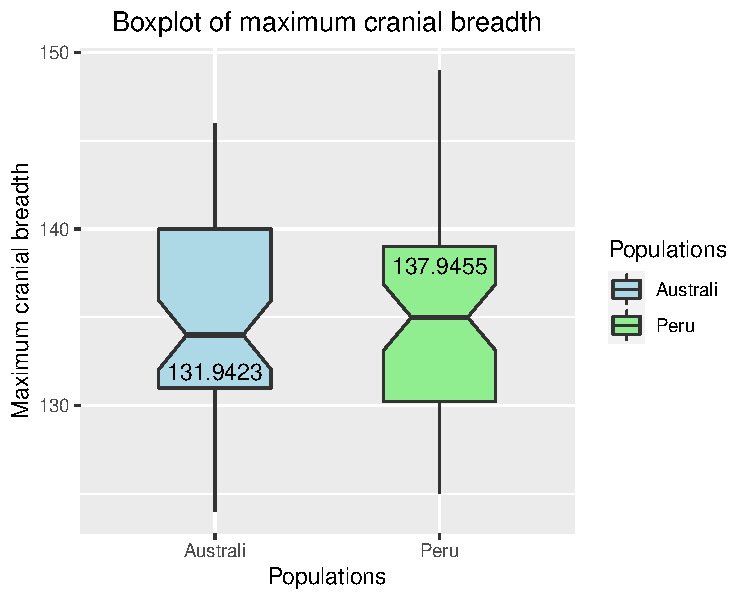
\includegraphics[width=\maxwidth]{figure/unnamed-chunk-7-1} 

}

\end{Schunk}
Boxplot represent maximum cranial breadth of Austali and Peru with the arithmetic average of each population placed on each box. X-axis shows the population and y-axis show the number of maximum cranial breadth.\\

\begin{center}
\textbf {Histograms represent maximum cranial breadth of each population} \\
\end{center}
Histograms show frequency of maximum cranial breadth of Australi(on the left) and Peru(on the right) with the number of frequency on top of each bar. X-axis shows the number of maximum cranial breadth and y-axis shows the frequency.\\
\begin{Schunk}

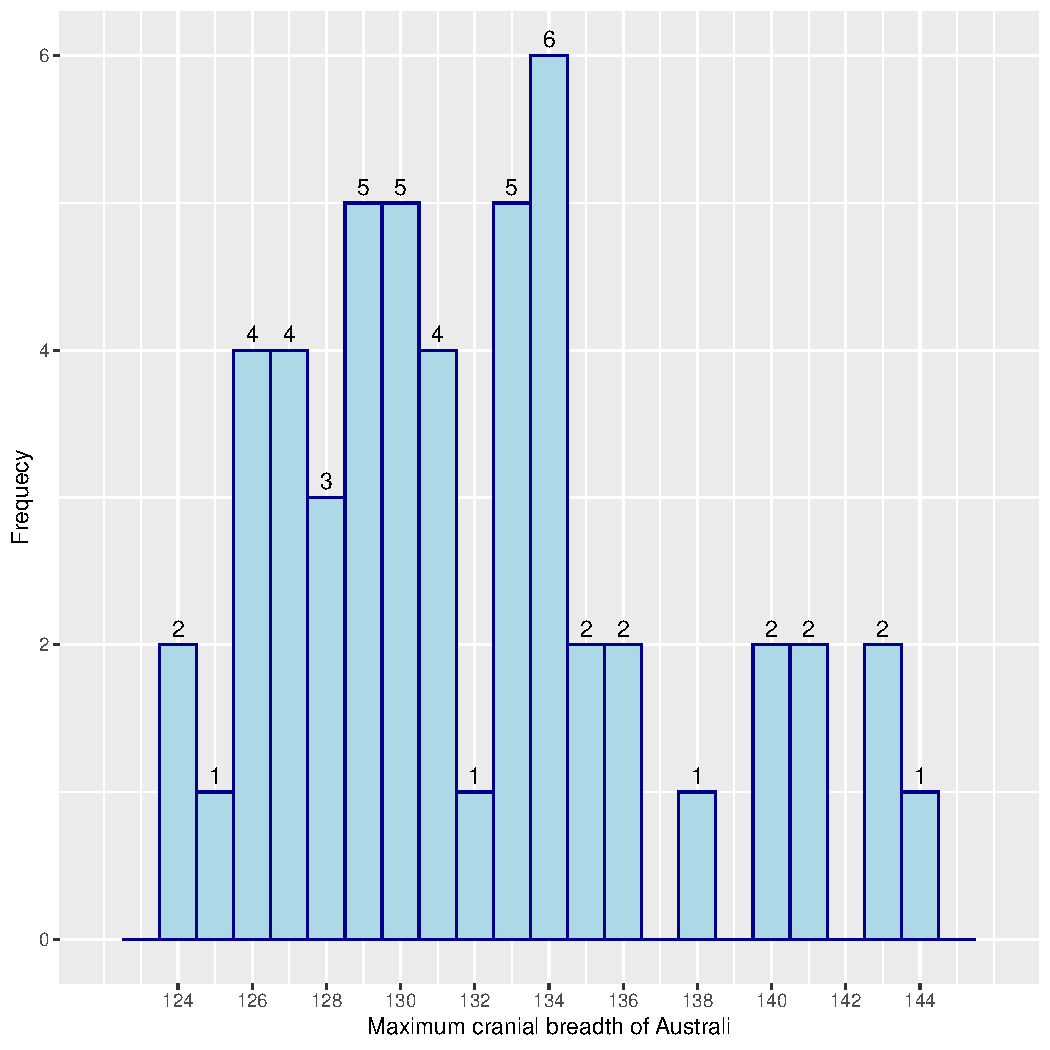
\includegraphics[width=8cm,height=8cm]{figure/unnamed-chunk-8-1} 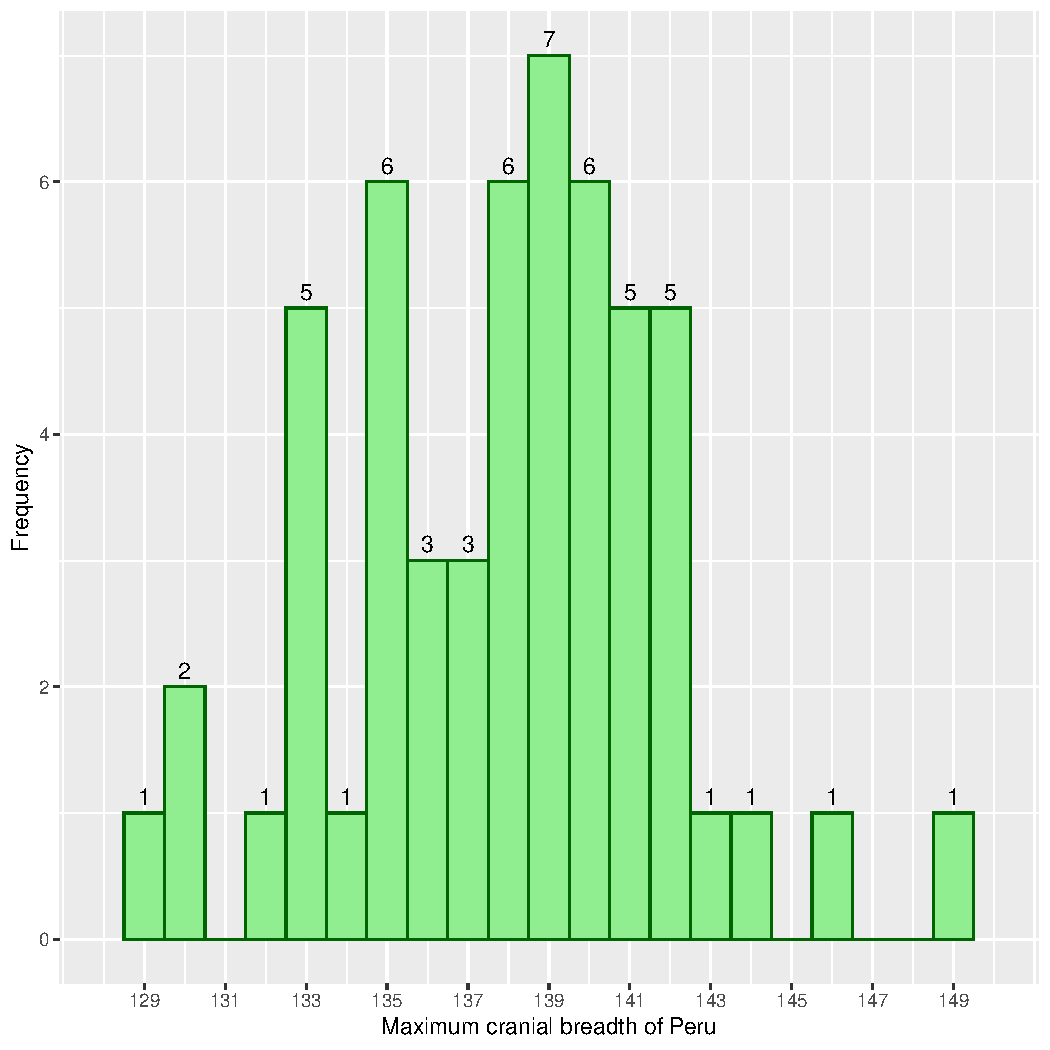
\includegraphics[width=8cm,height=8cm]{figure/unnamed-chunk-8-2} \end{Schunk}
\newpage
\begin{center}
\textbf {QQ-plot represent maximum cranial breadth of each population} \\
\end{center}
The left figure shows qq-plot represent maximum cranial breadth of Australi while the right one is for Peru. \\
\begin{Schunk}

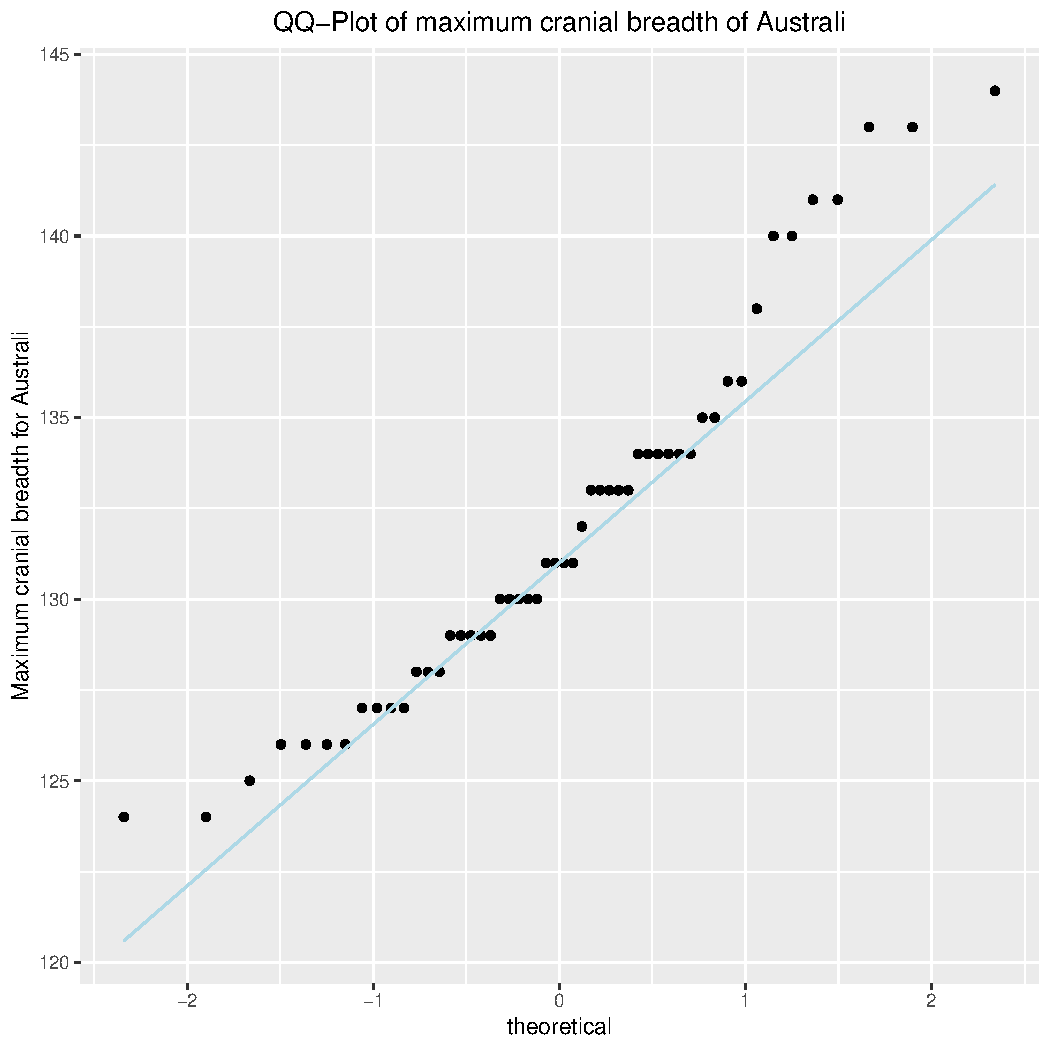
\includegraphics[width=8cm,height=8cm]{figure/unnamed-chunk-9-1} 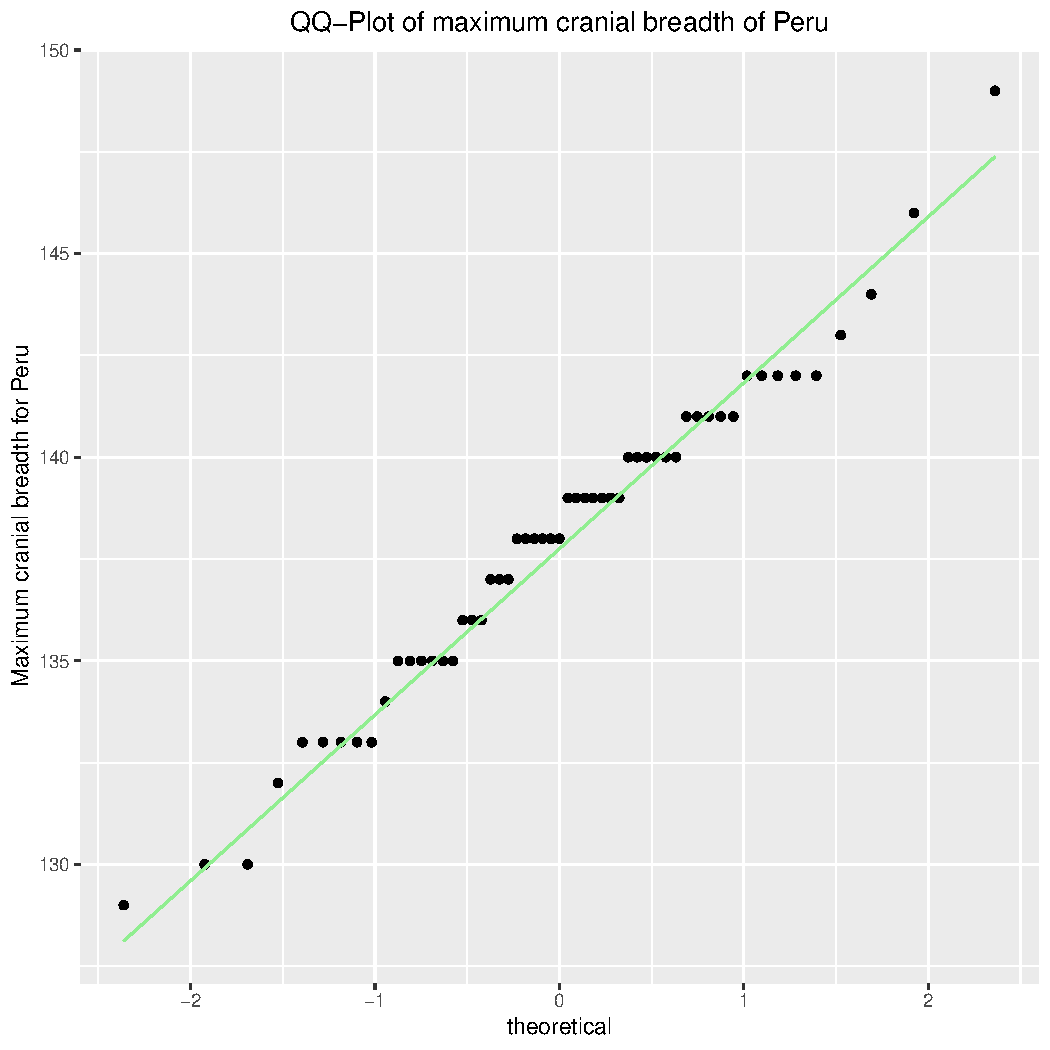
\includegraphics[width=8cm,height=8cm]{figure/unnamed-chunk-9-2} \end{Schunk}

\section*{Exercise 2}
\noindent 1. Calculate the number of men and women in Spain for each year and print them in a table together with the total population.

\subsection*{Implementation in R}
\begin{Schunk}
\begin{Sinput}
setwd(getwd())
Spanish.province <- read.csv('area_spanish_provinces.csv')
Spanish.population <- read.csv('population-spain-1998-2018.csv', sep=";")

population.2018 <- sum(Spanish.population$males.2018, Spanish.population$females.2018)
population.2013 <- sum(Spanish.population$males.2013, Spanish.population$females.2013)
population.2008 <- sum(Spanish.population$males.2008, Spanish.population$females.2008)
population.2003 <- sum(Spanish.population$males.2003, Spanish.population$females.2003)
population.1998 <- sum(Spanish.population$males.1998, Spanish.population$females.1998)

total.population <- sum(colSums(Spanish.population[ ,-1]))

population.df <- data.frame(Male=c(sum(Spanish.population$males.1998), 
                                   sum(Spanish.population$males.2003), 
                                   sum(Spanish.population$males.2008), 
                                   sum(Spanish.population$males.2013), 
                                   sum(Spanish.population$males.2018), 0),
                 Female=c(sum(Spanish.population$females.1998), 
                          sum(Spanish.population$females.2003), 
                          sum(Spanish.population$females.2008), 
                          sum(Spanish.population$females.2013), 
                          sum(Spanish.population$females.2018), 0),
                 Total=c(population.1998, population.2003, 
                         population.2008, population.2013, 
                         population.2018, total.population))

row.names(population.df) <- c('1998', '2003', '2008', '2013', '2018', 'Total')
population.df[6,1] <- sum(population.df$Male)
population.df[6,2] <- sum(population.df$Female)
\end{Sinput}
\end{Schunk}

\noindent 2. Display barplot plot of total population of Spain in each of the years, with each bar divided
between men and women.

\subsection*{Implementation in R}
\begin{Schunk}
\begin{Sinput}
library(ggplot2)
year <- c(1998, 1998, 2003, 2003, 2008, 2008, 2013, 2013, 2018, 2018)
population <- c(sum(Spanish.population$males.1998), 
                sum(Spanish.population$females.1998), 
                sum(Spanish.population$males.2003), 
                sum(Spanish.population$females.2003), 
                sum(Spanish.population$males.2008), 
                sum(Spanish.population$females.2008), 
                sum(Spanish.population$males.2013), 
                sum(Spanish.population$females.2013), 
                sum(Spanish.population$males.2018), 
                sum(Spanish.population$females.2018))
options(scipen = 999)
gender <- c('Male', 'Female', 'Male', 'Female', 'Male', 
            'Female', 'Male', 'Female', 'Male', 'Female' )

df.population <- data.frame(year, population, gender)
population.barplot<-ggplot(data=df.population, 
                           aes(x=year, y=population, fill=gender )) +
                    geom_col() +
                    scale_fill_manual(values=c("lightpink", "lightblue")) +
                    scale_x_continuous(breaks = seq(1998, 2018, 5)) + 
                    scale_y_continuous(breaks = seq(0, 50000000, 5000000)) +
                    geom_text(aes(label = sprintf("%.0fk", population/1000)), 
                              position = position_stack(0.5)) +
                    theme(axis.text.y=element_text(angle = 45))
\end{Sinput}
\end{Schunk}

\noindent 3. Display barplot of relative proportions of men and women within each province in 2018
\subsection*{Implementation in R}
\begin{Schunk}
\begin{Sinput}
proportion.province <-c(as.vector(Spanish.population$province), as.vector(Spanish.population$province))
proportion.gender <- c(rep('Male', 52), rep('Female', 52))
proportion.male <- round(Spanish.population$males.2018 / (Spanish.population$males.2018 + Spanish.population$females.2018), 4)
proportion.female <- round(Spanish.population$females.2018 / (Spanish.population$males.2018 + Spanish.population$females.2018), 4)

proportion.province.gender <- c(proportion.male, proportion.female)

df.proportion <- data.frame(Provinces=proportion.province, 
                            Proportion=proportion.province.gender, 
                            Gender=proportion.gender)

proportion.barplot <- ggplot(data=df.proportion, 
                             aes(x=Provinces, y=Proportion, fill=Gender)) + 
                      geom_col() + 
                      theme(axis.text.x=element_text(angle = 90, size=6), 
                            plot.title = element_text(vjust=0.5, hjust=1)) +
                      scale_fill_manual(values=c("lightpink", "lightblue")) +
                      scale_x_discrete(name= "Provinces") +
                      scale_y_continuous(name= "Population proportion")
\end{Sinput}
\end{Schunk}

\noindent 4. Calculate population density in each province in 1998 and in 2018.
\subsection*{Implementation in R}
\begin{Schunk}
\begin{Sinput}
province.population.2018 <- Spanish.population$males.2018 + Spanish.population$females.2018
province.population.1998 <- Spanish.population$males.1998 + Spanish.population$females.1998
provinces <- sapply(strsplit(as.vector(Spanish.population$province), ", "), '[', 1)

df <- data.frame(province = provinces, 
                 population.1998 = province.population.1998, 
                 population.2018 =province.population.2018)

area.provinces <- sapply(strsplit(as.vector(Spanish.province$Province)," "), tail, 1)
df1 <- data.frame(province = area.provinces, area = Spanish.province$Area)

for(i in 1:52){
  for(j in 1:52){
    if(grepl(df1$province[j], df$province[i])){
      df$area[i] <- df1$area[j]
    }
  }
}

df$province <- Spanish.population$province
df$density.1998 <- round(df$population.1998 / df$area, 4)
df$density.2018 <- round(df$population.2018 / df$area, 4)

density.2018.sample_size <- length(df$density.2018)
density.2018.sample_mean <- cal_mean(df$density.2018)
density.2018.sample_five_num_summary <- cal_five_num_summary(df$density.2018)
density.2018.sample_skewness <- cal_coef_skew(df$density.2018)
density.2018.kurtosis <- cal_coef_kurt(df$density.2018)
density.2018.sample_sd <- cal_sd(df$density.2018)

density.1998.sample_size <- length(df$density.1998)
density.1998.sample_mean <- cal_mean(df$density.1998)
density.1998.sample_five_num_summary <- cal_five_num_summary(df$density.1998)
density.1998.sample_skewness <- cal_coef_skew(df$density.1998)
density.1998.kurtosis <- cal_coef_kurt(df$density.1998)
density.1998.sample_sd <- cal_sd(df$density.1998)

density.characteristics <- data.frame("1998"=c(density.1998.sample_size, 
                                               density.1998.sample_mean, 
                                               density.1998.sample_five_num_summary, 
                                               density.1998.sample_skewness, 
                                               density.1998.kurtosis, 
                                               density.1998.sample_sd),
                                      "2018"=c(density.2018.sample_size, 
                                               density.2018.sample_mean, 
                                               density.2018.sample_five_num_summary, 
                                               density.2018.sample_skewness, 
                                               density.2018.kurtosis, 
                                               density.2018.sample_sd),
                                      row.names = c('Size', 'Mean', 'Minimum', 
                                                    'Q1', 'Q2', 'Q3', 'Maximum', 
                                                    'Skewness', 'Kurtosis', 'Standard Deviation'))

colnames(density.characteristics) <- c("Year 1998", "Year 2018")

year.1998 <- rep('1998', 52)
year.2018 <- rep('2018', 52)
year <- c(year.1998, year.2018)
values <- c(df$density.1998, df$density.2018) 
density.df <- data.frame(year, values)

density.boxplot <- ggplot(density.df, aes(x=year, y=values, fill=year)) +
                  geom_boxplot(notch = TRUE) +
                  scale_fill_manual(values=c("lightblue", "lightgreen")) +
                  ylab('Population density') +
                  xlab('Year') +
                  ggtitle('Boxplot of population density in Spain') +
                  theme(plot.title = element_text(hjust = 0.5))

hist.1998 <- ggplot(data=df, aes(x=density.1998)) + 
                geom_histogram(color="darkblue", fill="lightblue", binwidth = 50) + 
                xlab('Population density in 1998') +
                ylab('Frequecy') +
                scale_x_continuous(breaks = seq(0, 5000, 500))

hist.2018 <- ggplot(data=df, aes(x=density.2018)) + 
                geom_histogram(color="darkgreen", fill="lightgreen", binwidth = 50) + 
                xlab('Population density in 2018') +
                ylab('Frequecy') +
                scale_x_continuous(breaks = seq(0, 7000, 500))

histogram.group <- ggplot(density.df, aes(x = values)) +
              geom_histogram(aes(color = year, fill = year), 
                            position = "identity", bins = 30, alpha = 0.4, binwidth = 50) +
              scale_color_manual(values = c("#00AFBB", "#E7B800")) +
              scale_fill_manual(values = c("#00AFBB", "#ffffff00")) +
              scale_x_continuous(breaks = seq(0, 7000, 500)) +
              xlab('Population density') +
              ylab('Frequecy')
\end{Sinput}
\end{Schunk}


\noindent 5. Interpretion of results and graphics. \\

\begin{center}
\textbf {Table of population in Spain} \\
\end{center}
Table represents the population of Spain in 1998, 2003, 2008, 2013 and 2018. It shows the total population based on gender between each year, the total population between each year, and the total population of the 5 selected year.

% latex table generated in R 3.6.3 by xtable 1.8-4 package
% Mon Apr 13 17:38:18 2020
\begin{table}[ht]
\centering
\begingroup\large
\begin{tabular}{|l|l|l|l|}
  \hline
 & Male & Female & Total \\ 
  \hline
1998 & 19488465 & 20364186 & 39852651 \\ 
  2003 & 21034326 & 21682738 & 42717064 \\ 
  2008 & 22847737 & 23310085 & 46157822 \\ 
  2013 & 23196386 & 23933397 & 47129783 \\ 
  2018 & 22896602 & 23826378 & 46722980 \\ 
  Total & 109463516 & 113116784 & 222580300 \\ 
   \hline
\end{tabular}
\endgroup
\caption{Population of Spain} 
\end{table}


\newpage
\begin{center}
\textbf {Barplot of population in Spain} \\
\end{center}
Barplot of total popuation in Spain in 1998, 2003, 2008, 2013 and 2018 with bar separated by gender. Male in blue and Female in pink. Each bar has two numbers represents total population based on gender in each year. X-axis shows the years and y-axis shows population. The number of population in Spain slightly increased till 2013 and slightly dropped in 2018.
\begin{Schunk}

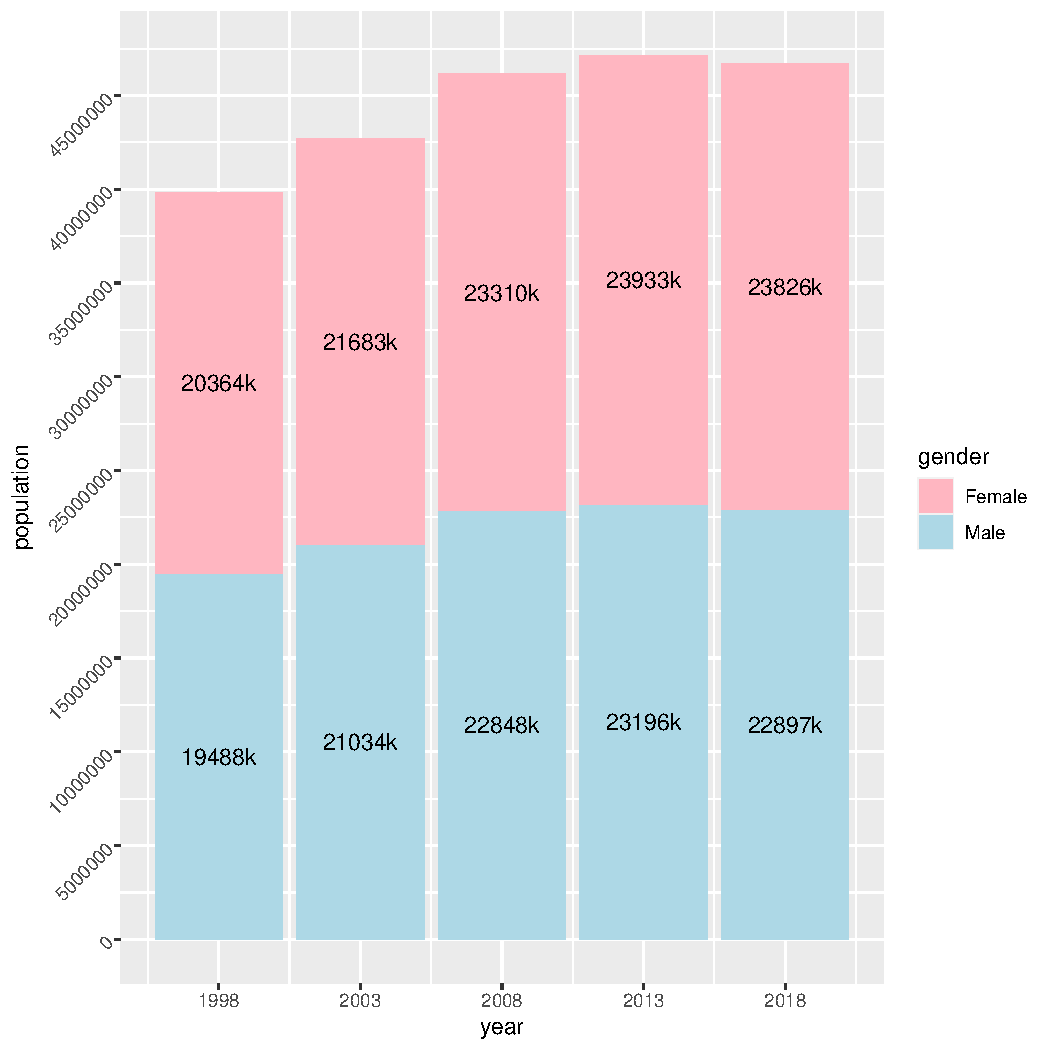
\includegraphics[width=\maxwidth]{figure/unnamed-chunk-15-1} \end{Schunk}

\newpage
\begin{center}
\textbf {Barplot of proportions of men and women in Spain (2018)} \\
\end{center}
Barplot represents population proportion of each province in Spain in 2018. X-axis shows provinces in Spain while y-axis show the relative proportion. Each bar is divided between men and women of each province. The blue part is for men and the pink part is for women. The proportion of men and women in each province is almost equal with men are slightly less than women.
\begin{Schunk}

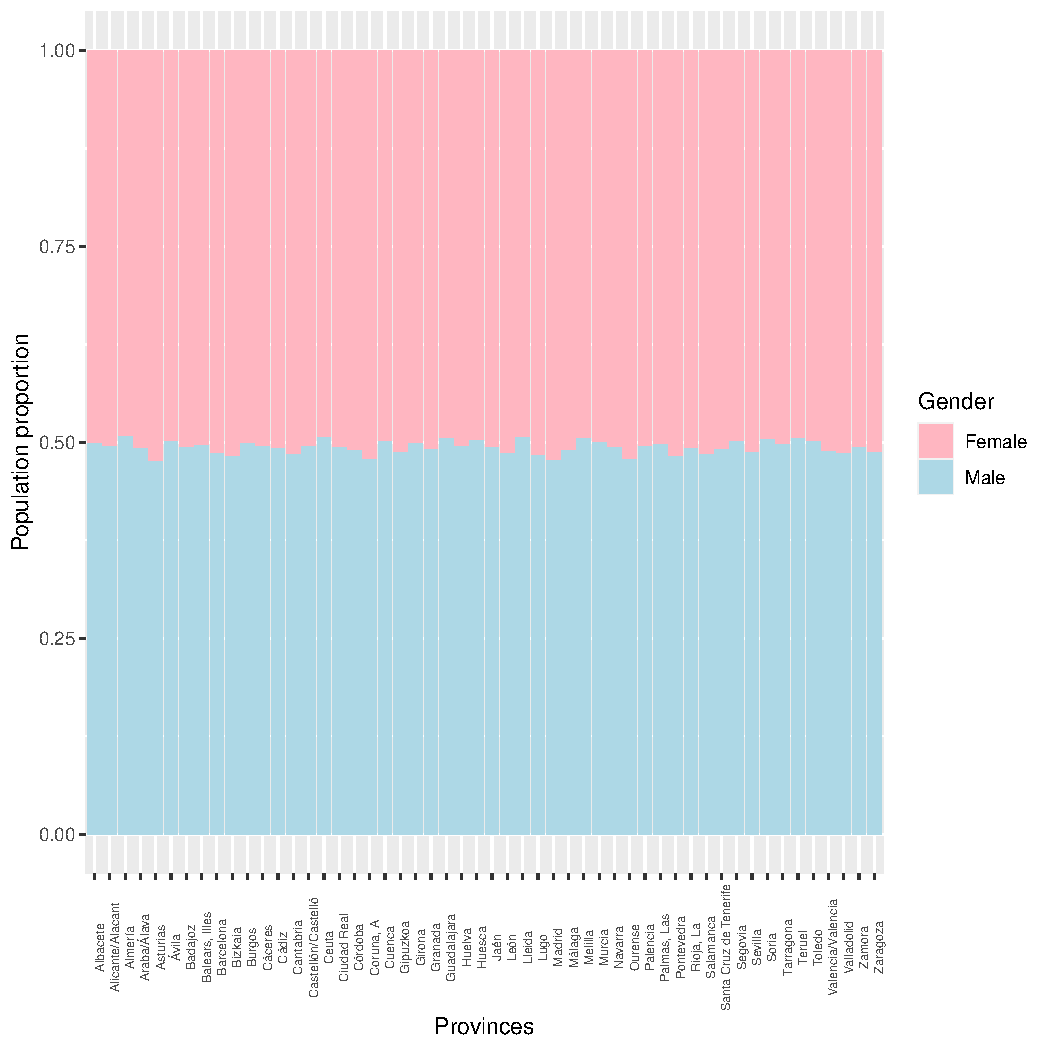
\includegraphics[width=\maxwidth]{figure/unnamed-chunk-16-1} \end{Schunk}

\newpage
\begin{center}
\textbf {Table of characteristics of population density in Spain (1998 and 2018)}
\end{center}

% latex table generated in R 3.6.3 by xtable 1.8-4 package
% Mon Apr 13 17:38:19 2020
\begin{table}[ht]
\centering
\begin{tabular}{|l|l|l|}
  \hline
 & Year 1998 & Year 2018 \\ 
  \hline
Size &   52.0000 &   52.0000 \\ 
  Mean &  268.3568 &  339.0729 \\ 
  Minimum &    8.8899 &    8.5994 \\ 
  Q1 &   26.5034 &   26.4518 \\ 
  Q2 &   55.7095 &   64.1000 \\ 
  Q3 &  154.2437 &  188.0495 \\ 
  Maximum & 4623.6923 & 6644.9231 \\ 
  Skewness &    4.5286 &    4.7737 \\ 
  Kurtosis &   19.7477 &   22.5997 \\ 
  Standard Deviation &  812.2020 & 1089.5388 \\ 
   \hline
\end{tabular}
\caption{Characteristics of Population density of Spain} 
\end{table}


\begin{Schunk}


{\centering 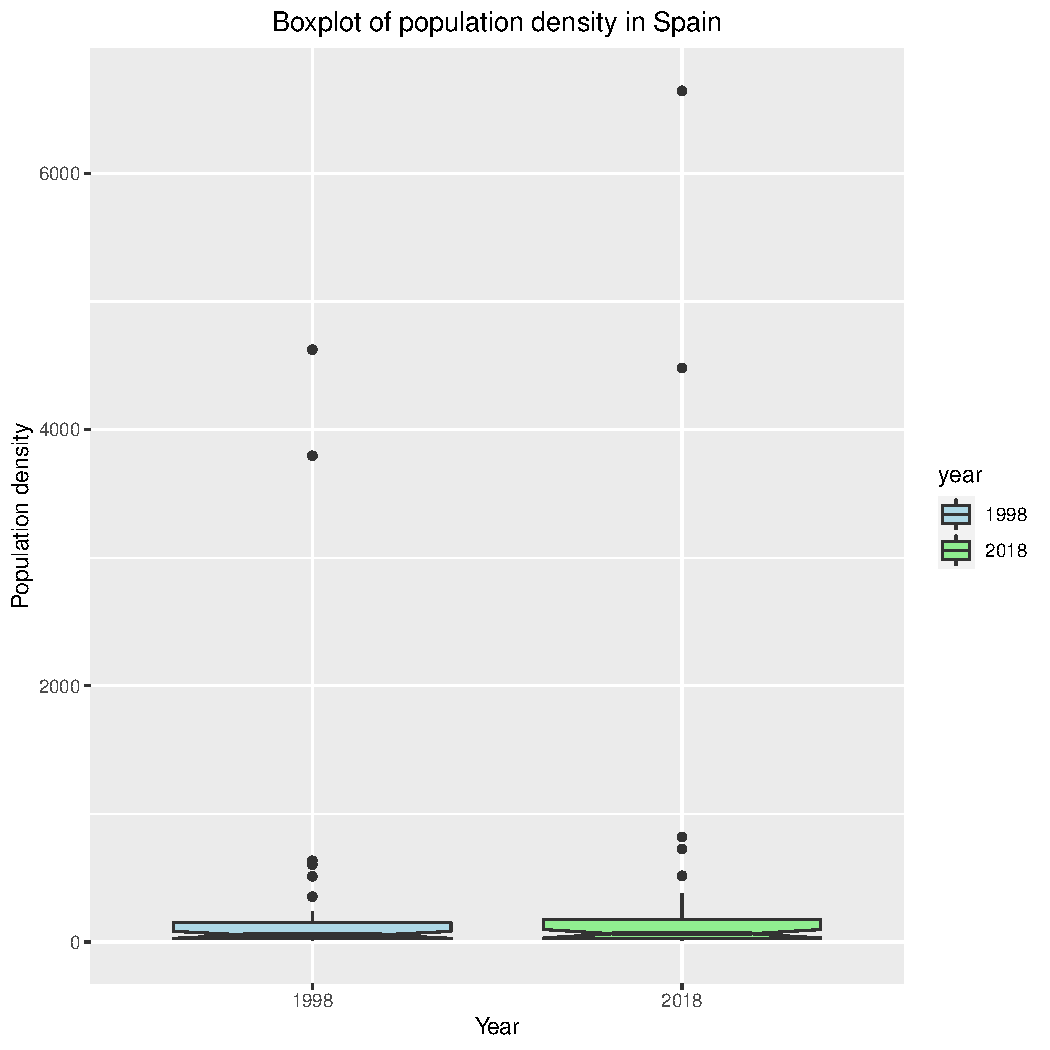
\includegraphics[width=15cm,height=15cm]{figure/unnamed-chunk-18-1} 

}

\end{Schunk}


\begin{center}
\textbf {Histograms represent population density in Spain} \\
\end{center}
First two histograms show population density in Spain in 1998 and 2018. The x-axis shows population density while the y-axis shows frequency. The last histogram shows the joining of population density in Spain in 1998 and 2018.\\

\begin{Schunk}


{\centering 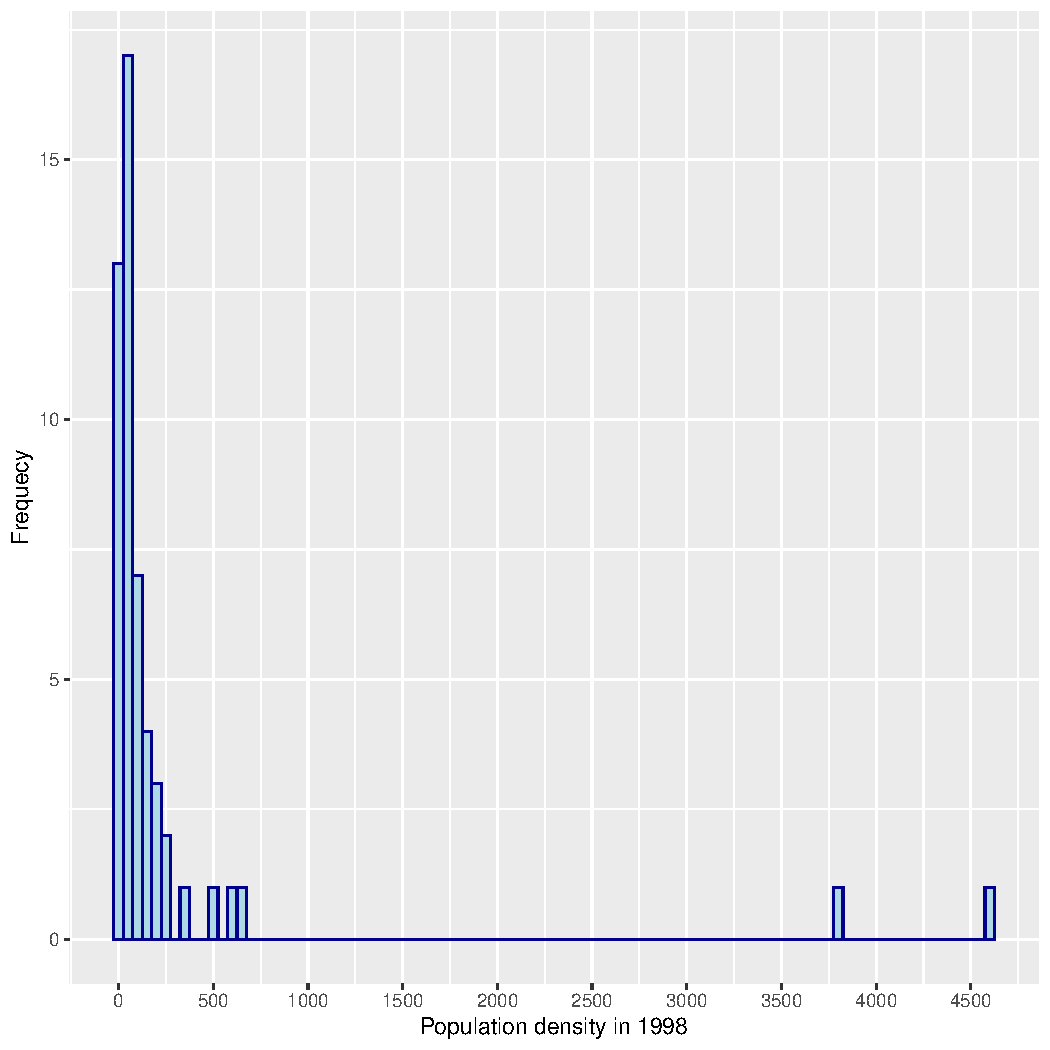
\includegraphics[width=8cm,height=8cm]{figure/unnamed-chunk-19-1} 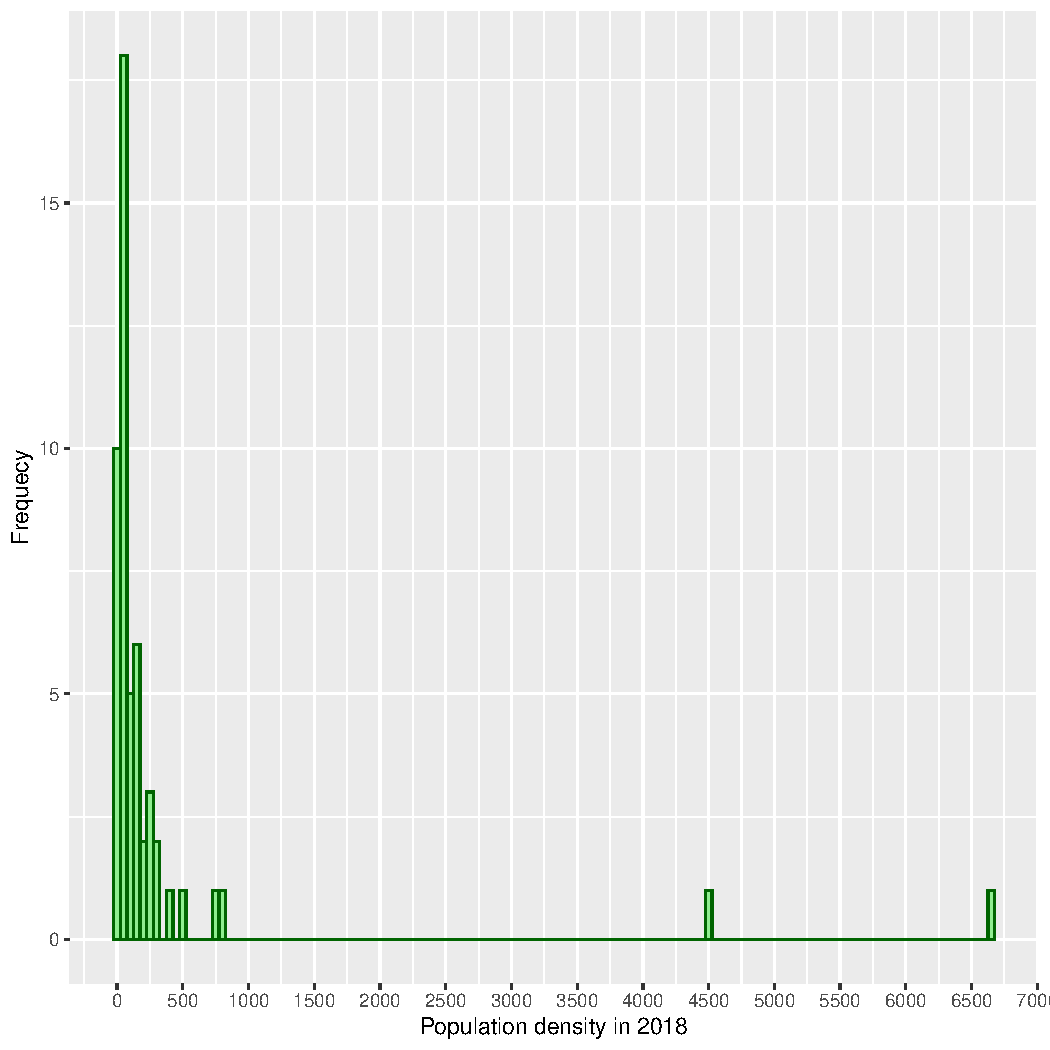
\includegraphics[width=8cm,height=8cm]{figure/unnamed-chunk-19-2} 

}

\end{Schunk}

\begin{Schunk}


{\centering 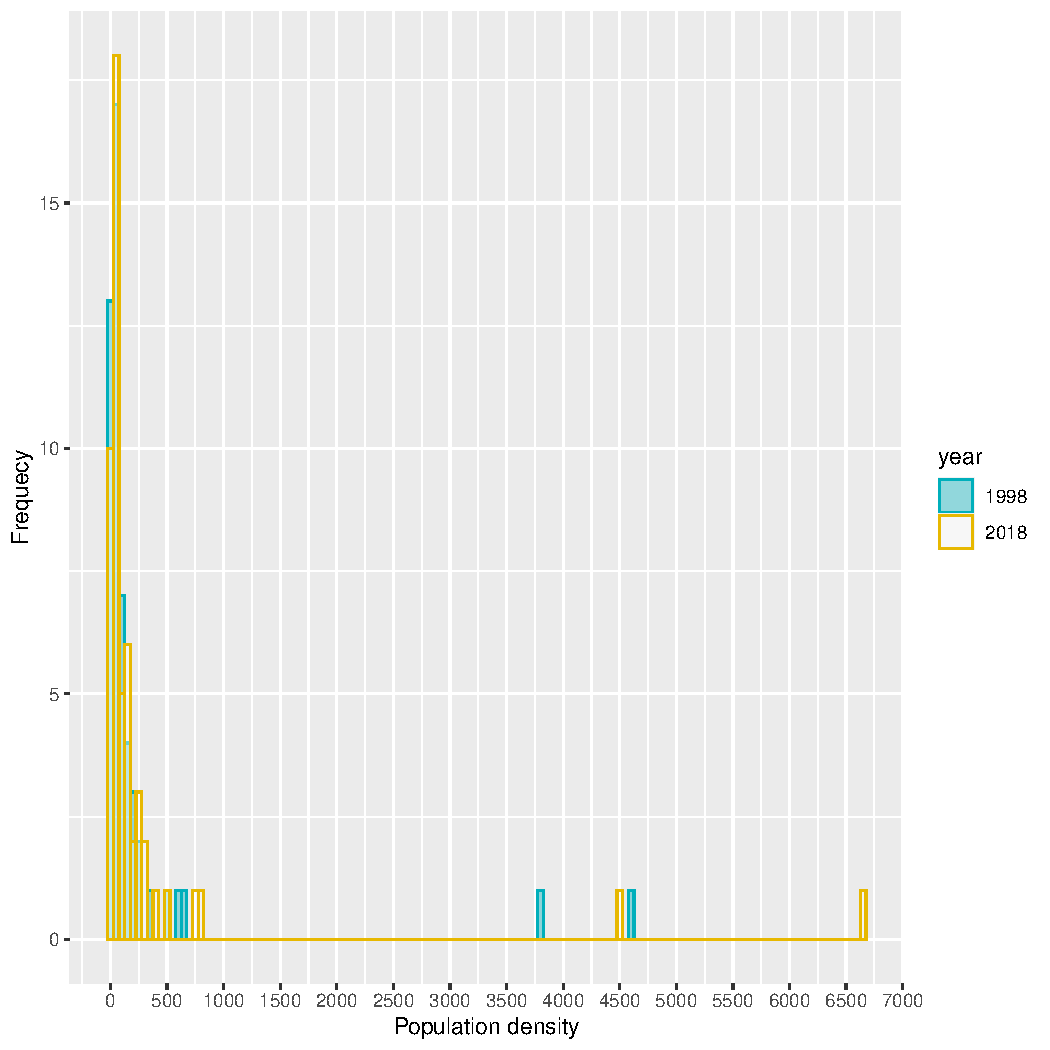
\includegraphics[width=16cm,height=12cm]{figure/unnamed-chunk-20-1} 

}

\end{Schunk}

\end{document}

